\documentclass[10pt,conference]{IEEEtran}

\usepackage[utf8]{inputenc}
\usepackage{graphicx}
\usepackage{url}
\usepackage{enumitem}
\usepackage{float}

\title{1st Lab with VTK (Visualization Tool Kit)}

\author{
\IEEEauthorblockN{João Varela, 113780}
\IEEEauthorblockN{Carolina Prata, 114246}
\IEEEauthorblockA{Information Visualization, 2025\\
MSc in Computer Engineering, University of Aveiro}
}

\begin{document}

\maketitle

\begin{abstract}
This document provides an overview of the work carried out during the first laboratory session of the Information Visualization course, whose purpose was to gain an initial understanding of the VTK framework.
\end{abstract}

\section{Introduction}
The Visualization Toolkit (VTK) is an open-source software framework extensively used in 3D computer graphics, image processing, and scientific visualization. It offers a robust collection of tools for constructing, modifying, and rendering complex visual representations. VTK handles numerous data types and supports various visualization methods, including volume rendering, contouring, and streamline analysis.

\section{Development}

The laboratory assignment provided by the course instructor comprises several exercises covering the following topics:

\begin{itemize}
    \item VTK installation;
    \item First VTK example and the visualization pipeline;
    \item VTK interactors;
    \item Camera control;
    \item Lighting;
    \item Actor properties;
    \item Final exercise.
\end{itemize}


\subsection{VTK installation}
For this exercise, it was only required to install VTK in our local machine, and for that we used \texttt{pip} inside a virtual environment. The \texttt{requirements.txt} file includes the required \texttt{vtk} package.
The commands executed were:

\begin{verbatim}
python3 -m venv venv
source venv/bin/activate
pip install -r requirements.txt
\end{verbatim}

\subsection{First VTK example and the visualization pipeline}
In this section, several introductory exercises are provided. The first task consists of downloading and running the file cone.py, which contains Python code illustrating a basic visualization example using VTK. When executed, the script generates the following output:

%IMAGEM CONE INICIAL
\begin{figure}[H]
\centering
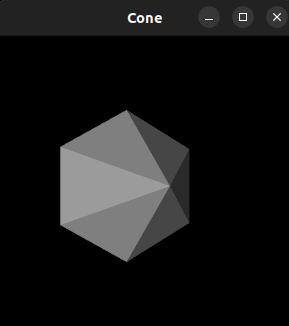
\includegraphics[width=0.25\textwidth]{lesson1/fig1.png}
\caption{Result of executing the \texttt{cone.py} example.}
\label{fig:cone}
\end{figure}

In this exercise, we were asked to modify the cone defined in \texttt{cone.py} by adjusting its geometric parameters. Specifically, we updated the code to set the cone's height to 2 and its radius to 1, using the following instructions:

\begin{verbatim}
coneSource.SetHeight(2)
coneSource.SetRadius(1)
\end{verbatim}

Additionally, we were instructed to run several tests by applying different values to \texttt{SetResolution}, allowing us to observe how changes in resolution affect the visual representation of the cone. Here are some example outputs obtained during these tests.

\begin{figure}[H]
\centering

% Linha de cima
\begin{minipage}{0.28\linewidth}
    \centering
    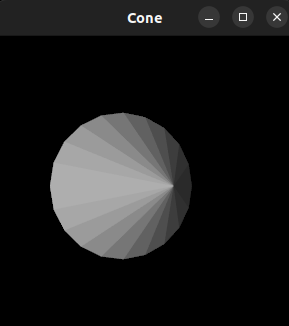
\includegraphics[width=\linewidth]{lesson1/fig2_20.png}
\end{minipage}
\hspace{0.5cm}
\begin{minipage}{0.28\linewidth}
    \centering
    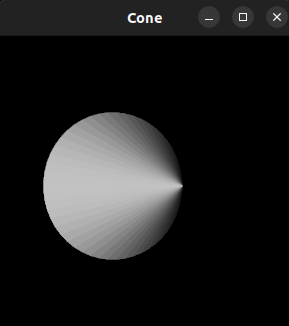
\includegraphics[width=\linewidth]{lesson1/fig2_100.png}
\end{minipage}

\vspace{0.4cm}

% Linha de baixo (centrada)
\begin{minipage}{0.28\linewidth}
    \centering
    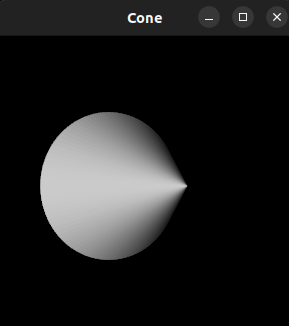
\includegraphics[width=\linewidth]{lesson1/fig2_50.png}
\end{minipage}

\caption{Cones with resolutions of 20, 50 and 100.}
\label{fig:resolutions}
\end{figure}


The SetResolution method is used to control the number of facets used to approximate the cone’s circular base, effectively defining how smooth or coarse the cone appears in the rendered visualization.

It was also requested to change the background color of the rendering window to white. This was achieved by applying the \texttt{SetBackground(1,1,1)} method to the renderer.
\begin{figure}[H]
\centering
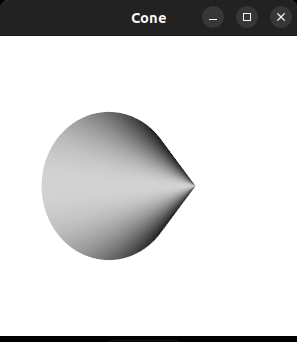
\includegraphics[width=0.25\textwidth]{lesson1/fig3.png}
\caption{Cone with the background changed to white}
\label{fig:cone}
\end{figure}

The final exercise consisted of modifying the size of the visualization window and determining its default dimensions. To achieve this, we added the instruction \texttt{renWin.SetSize(x, y)}, where \texttt{x} and \texttt{y} define the desired window width and height. We tested the sizes \texttt{300×300}, \texttt{400×400} and \texttt{500×500}, and observed that the default window size corresponds to \texttt{300×300}.

In this exercise, we were asked to extend the original code by adding two additional geometric primitives: a sphere and a cylinder. The sphere was implemented using \texttt{vtkSphereSource} with a radius of 2, while the cylinder was created through \texttt{vtkCylinderSource} with a radius of 2 and a height of 3.

\begin{figure}[H]
\centering

\begin{minipage}{0.45\columnwidth}
    \centering
    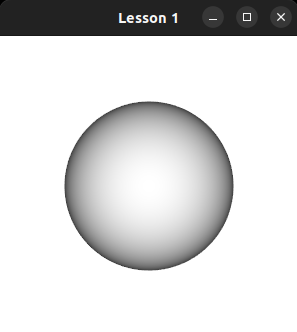
\includegraphics[width=\linewidth]{lesson1/fig4_esfera.png}
\end{minipage}
\hfill
\begin{minipage}{0.45\columnwidth}
    \centering
    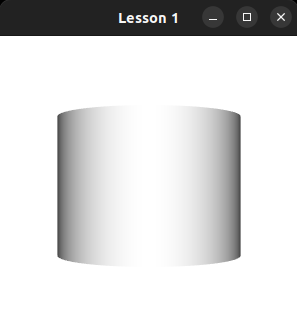
\includegraphics[width=\linewidth]{lesson1/fig4_cilindro.png}
\end{minipage}

\caption{Sphere and Cylinder}
\label{fig:sphere_cylinder}
\end{figure}

\subsection{VTK Interactors}
In this section, we were instructed to explore the interactor provided by the VTK package. For this purpose, we replicated the previous example into a new file named \texttt{interaction.py}, and added the following lines:

\begin{verbatim}
iren = vtkRenderWindowInteractor()
iren.SetRenderWindow(renWin)
iren.Initialize()
iren.Start()
\end{verbatim}
All the interaction controls listed in the assignment README were tested, and we confirm that their behavior matches the expected effects.

\begin{figure}[H]
\centering
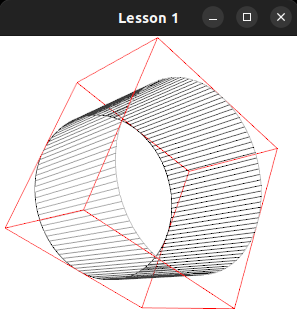
\includegraphics[width=0.25\textwidth]{lesson1/fig5.png}
\caption{Example of interactions (Wireframe and Pick).}
\label{fig:cone}
\end{figure}


\subsection{Camera Control}
In this section, we explored different aspects of camera control in VTK. For this purpose, we replicated the previous example into a new file named \texttt{camera.py}. Following the instructions, we added the provided camera configuration code immediately after creating the renderer:

\begin{verbatim}
cam1 = vtkCamera()
cam1.SetPosition(10,0,0)
cam1.SetViewUp(0,1,0)
ren.SetActiveCamera(cam1)
\end{verbatim}

We then modified the camera parameters by setting the \textit{Position} to (10, 10, 0) and the \textit{View Up} vector to (0, 1, 1). After applying these changes, the visualization adjusted accordingly, producing a slightly oblique view of the cylinder. By further experimenting with different camera positions and orientations, we verified how each parameter affects perspective, depth, and the overall perception of the rendered scene.
\begin{figure}[H]
\centering

\begin{minipage}{0.45\columnwidth}
    \centering
    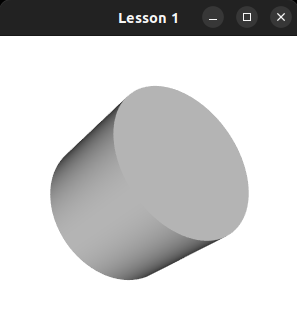
\includegraphics[width=\linewidth]{lesson1/fig6_1.png}
\end{minipage}
\hfill
\begin{minipage}{0.45\columnwidth}
    \centering
    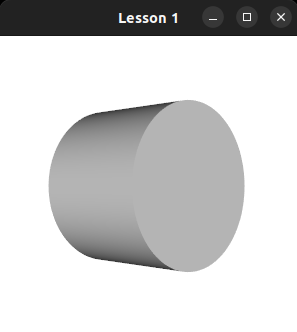
\includegraphics[width=\linewidth]{lesson1/fig6_2.png}
\end{minipage}

\caption{Different views of the camera, the first one with the vector (0,1,1) and the second one with the (0,0,2)}
\label{fig:sphere_cylinder}
\end{figure}


In this part of the exercise, instead of creating a new camera using
\texttt{cam1 = vtkCamera()}, we were instructed to retrieve the default
camera created by the renderer. This was done by replacing that line with
\texttt{cam1 = ren.GetActiveCamera()}, allowing us to modify the existing
camera rather than creating a new instance.

Afterwards, we enabled the orthographic projection mode using
\texttt{cam1.SetParallelProjection(True)} and visualized a cube in wireframe.
Switching between perspective and orthographic projection revealed clear
differences: in orthographic mode, the cube is rendered without perspective
distortion, and its parallel edges remain parallel regardless of distance.
\begin{figure}[H]
\centering
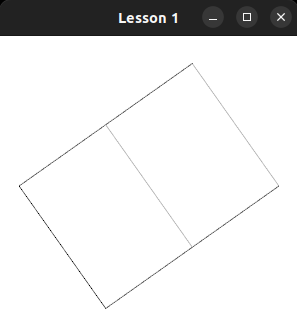
\includegraphics[width=0.25\textwidth]{lesson1/fig7.png}
\caption{Cube (wireframe) in paralel projection.}
\label{fig:cone}
\end{figure}


\subsection{Lighting}

This section focused on experimenting with lighting in VTK. For this purpose, we replicated the previous example into a new file named \texttt{lightning.py}.
To achieve this, we introduced a new light source and configured it based on the camera's parameters.  
The following lines were added to create a red light, position it at the camera's location, and attach it to the renderer:

\begin{verbatim}
cam1 = ren.GetActiveCamera()
light = vtkLight()
light.SetColor(1,0,0)
light.SetFocalPoint(cam1.GetFocalPoint())
light.SetPosition(cam1.GetPosition())
ren.AddLight(light)
\end{verbatim}

\begin{figure}[H]
\centering

\begin{minipage}{0.45\columnwidth}
    \centering
    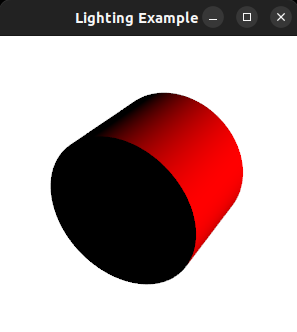
\includegraphics[width=\linewidth]{lesson1/fig8.png}
\end{minipage}
\hfill
\begin{minipage}{0.45\columnwidth}
    \centering
    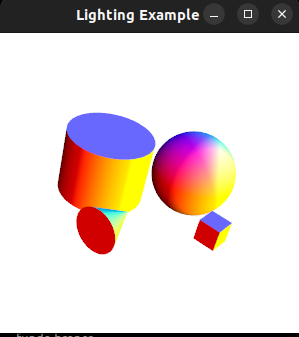
\includegraphics[width=\linewidth]{lesson1/fig8_2.png}
\end{minipage}

\caption{Examples of lights in different shapes.}
\label{fig:sphere_cylinder}
\end{figure}
The second image shows the scene illuminated with multiple light sources of different colors. We applied four lights: red, green, yellow, and blue, using all the geometric figures created so far to observe the combined lighting effects.

\subsection{Actor Properties}

It was also requested to modify the visual properties of an actor.
For this purpose, we used the original \texttt{cone.py} file and created a new file named \texttt{actors.py}.
To do this, we adjusted both the color and the opacity of the cone using the following code instructions:

\begin{verbatim}
coneActor.GetProperty().SetColor(0.2, 0.63, 0.79)
coneActor.GetProperty().SetOpacity(1)
\end{verbatim}

These changes allow the actor to be rendered with a customized color and transparency level, giving finer control over the object's appearance.

\begin{figure}[H]
\centering

% Linha de cima
\begin{minipage}{0.28\linewidth}
    \centering
    
\includegraphics[width=\linewidth]{lesson1/fig9_0.png}
\end{minipage}
\hspace{0.5cm}
\begin{minipage}{0.28\linewidth}
    \centering
    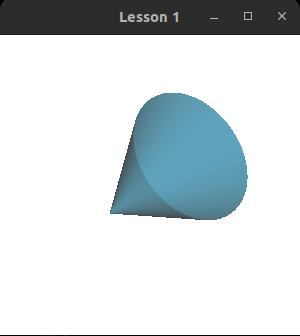
\includegraphics[width=\linewidth]{lesson1/fig9_05.png}
\end{minipage}

\vspace{0.4cm}

% Linha de baixo (centrada)
\begin{minipage}{0.28\linewidth}
    \centering
    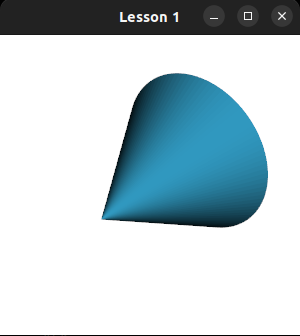
\includegraphics[width=\linewidth]{lesson1/fig9_color.png}
\end{minipage}

\caption{Cone visualization with the applied color and opacity settings (0, 0.5, 1).}
\label{fig:resolutions}
\end{figure}

\subsection{Last Exercise}

In the final exercise, we were asked to construct a multi–light environment by adding four colored light sources, each positioned in a different location in the 3D space and all directed towards the origin. The required lights were:

\begin{itemize}
    \item Red light at position $(-5, 0, 0)$,
    \item Green light at position $(0, 0, -5)$,
    \item Blue light at position $(5, 0, 0)$,
    \item Yellow light at position $(0, 0, 5)$.
\end{itemize}

To avoid code repetition, we implemented a function \texttt{create\_light\_with\_sphere(renderer, color, position)} that receives a color and a position, creates a \texttt{vtkLight} oriented towards the origin using \texttt{SetFocalPoint(0,0,0)}, and places a small sphere at the corresponding coordinates to visually represent the light’s location. These spheres were assigned a radius of $0.5$ and lighting was disabled through \texttt{actor->GetProperty()->SetLighting(False)} so that they preserve their true color and are not affected by other light sources.

To observe the combined effect of the four lights, we placed two different primitives at the center of the scene: first a sphere (with radius 2), and later a cone (with height 2 and radius 1). The images included below illustrate the visual differences between these two central objects when illuminated by the same multi–light configuration.

The results show how each surface reacts to directional colored lighting coming from four distinct positions. The sphere exhibits smooth shading transitions between colors, while the cone produces stronger contrasts due to its polygonal structure. In both cases, the colored spheres representing the lights retained their pure red, green, blue, and yellow tones, confirming that disabling lighting for these actors worked as intended.

\begin{figure}[H]
\centering
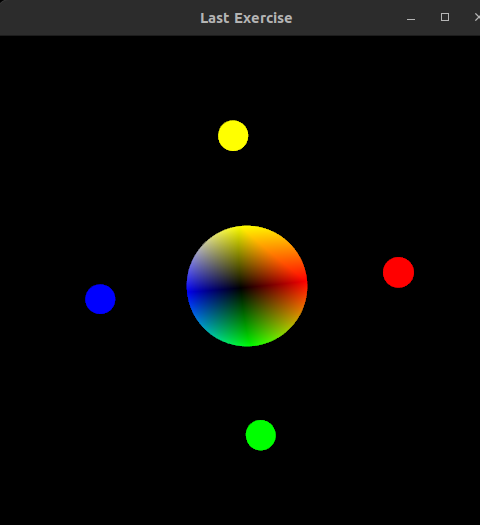
\includegraphics[width=0.25\textwidth]{lesson1/last_sphere.png}
\caption{Scene illuminated by four colored lights using a sphere as the central object.}
\label{fig:last_sphere}
\end{figure}

\begin{figure}[H]
\centering
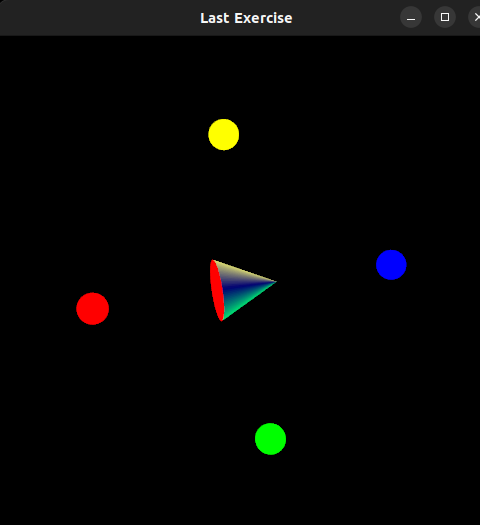
\includegraphics[width=0.25\textwidth]{lesson1/last_cone.png}
\caption{Attempt to replicate the reference example \texttt{lighting.png} using a cone as the central object under the same multi–light configuration.}
\label{fig:last_cone}
\end{figure}


\end{document}
